\scanpage{40}

\diagram{\begin{tikzcd}[ampersand replacement=\&,column sep=small]
\& X\arrow[d] \& \\
S \& T\arrow[l,"f" description] \& X\times_S S'\arrow[ul]\arrow[d]\\
\deleted{\unsure{S}}S'\arrow[u] \& \& S'\times_S T=T'\arrow[ll]\arrow[ul]\arrow[u,bend right=32]\arrow[ll,shift left=3,shorten >=1.1cm,shorten <=.7cm,"\unsure{f'}"]
\end{tikzcd}}

\figure{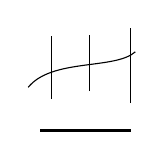
\begin{tikzpicture}[x=1cm,y=1cm]\draw[thin] (0,-.4)--(0,.4) (.48,-.3)--(.48,.42) (1,-.45)--(1,.5);\draw (-.3,-.25) .. controls (0,.12) and (.8,-.03) .. (1.06,.2);\draw[thick] (-.15,-.8)--(1,-.8);\end{tikzpicture}}

\diagram{\begin{tikzcd}[ampersand replacement=\&,column sep=small,row sep=small]
\& X_s\arrow[d] \& \\
s \& T_s\arrow[l,dash] \&\\
\& \& X'_{s'}\arrow[uul]\arrow[dl]\\
s' \& T'_{s'}\arrow[l,dash]\arrow[uu]\arrow[ur,dashed,bend right=35] \&
\end{tikzcd}}

\uline{Proposition 2} Supposons que $f_*(X/T)$ existe, et que pour tt $s\in S$, \deleted{toute}\unsure{tte|toute} multisection de $X_s/T_s$ définie sur une extension finie \inserted{$k'$} [\unsure{quelc.}] de $k(s)$, soit ``contenue'' dans un ouvert \inserted{d'un} \deleted{\unsure{affine d'un}} $U_i\otimes_k k'$ ($U_i$, famille donnée). Alors $f_*(X/T)$ est réunion des $f_{i*}(U_i/T)$ (\inserted{où} $f_i=f\vert U_i$).

\margin{dans le cas ``fini''}

[On suppose $T$ et $X$ de type fini sur $S$]

En effet, \deleted{soit} il suffit de montrer que \deleted{tout} pt \deleted{fermé} de $f_*(X/T)$ \unsure{provient} \deleted{\illegible{1}} \unsure{d'un|un des} $f_{i*}(U_i/T)$. Un tel pt fermé est défini par un corps $K$ sur un $k(s)$, et une \inserted{multi}section définie sur $K$ de $X_s$ sur $T_s$. On peut \unsure{le|la} supposer \deleted{définie sur une} $K$ fini sur $k(s)$, : à cause des hyp. de finitude \unsure{faites dans le|faites dans la} : \deleted{\unsure{les}} premier cas. Il provient \unsure{donc ...|d'un ...}

% slanted
\margin{remplace prop. 2}

\deleted{\uline{Corollaire}}\inserted{\uline{Proposition} $2^{\mathrm{bis}}$} Supposons que tte \inserted{multi}section $X_s/T_s$ définie sur une extension finie (resp. quelconque) $k'$ de $k(s)$ soit contenue dans un ouvert \deleted{\uline{affine} \unsure{pris}} \inserted{d'}une famille $U_i$. Supposons que les $f_{i*}(U_i/T)$ existent, alors il en est de $=$ de $f_*(X/T)$.

% archive sheet number: 39
